\documentclass[11pt, a4paper, titlepage]{scrartcl}

\usepackage[utf8x]{inputenc}
\usepackage[frenchb]{babel}
\usepackage[T1]{fontenc}
\usepackage{graphicx}
\usepackage{hyperref}
\usepackage{float}

%\renewcommand{\familydefault}{\sfdefault}
%\usepackage[top = 2.54cm, bottom = 2.54cm, left=2.5cm, right=2.5cm]{geometry}

\titlehead{\centering
\includegraphics[width=\textwidth]{images/logo}}
\title{Projet Data Mining}
\author{Pierre \textsc{Turpin}, Jean-Marie \textsc{Comets}}
\date{\today}

\begin{document}

\maketitle
\tableofcontents
\newpage

Au vu des nombreux problèmes de "scaling" que nous pouvions rencontrer
avec le jeu de données prévu, l'intégralité de ce rapport repose sur
l'analyse d'un échantillon de données. Bien entendu, avant d'étudier les
données, nous avons mélangé le jeu de données et pris un échantillon fixe pour
l'ensemble de l'étude.

\section{Caractérisation du flux vidéo}

\subsection{Popularité}

En étudiant les différents indicateurs quantitatifs (attribus *\_count),
représentant le nombre de visionnages d'un flux, nous avons pu remarquer que
quasiment toutes celles-ci sont indépendantes, mis à part l'attribut
\textit{stream\_count}, qui ne représente que la somme du
\textit{embedded\_count} et du \textit{site\_count}. \\

Nous avons donc retiré cet attribut, pour pouvoir définir la notion de
\textbf{popularité} d'un flux, correspondant à une somme normalisée des
différents indicateurs. \\

Cet indicateur nous sert d'heuristique pour établir les différentes
catégorisations suivantes :

\subsection{Catégorisation}

Un seul attribut permettant de catégoriser les différents flux est disponible,
et ce uniquement à partir du jeu de données XML : \textit{subcategory}. En
remarquant que cet attribut concerne à la fois la catégorie du jeu et sa
plateforme, nous avons séparé ces deux informations. \\

Ainsi, dans la figure \ref{fig:main_consoles}, nous n'observons pas la
plateforme PC, qui devrait cependant regrouper beaucoup de flux (plateforme non
définie là où le type de jeu est bien défini). Cependant, nous pouvons
remarquer qu'entre les différentes consoles de jeu, c'est la plateforme \textbf{XBOX}
qui a le plus de succès. \\

\begin{figure}[h]
    \centering
    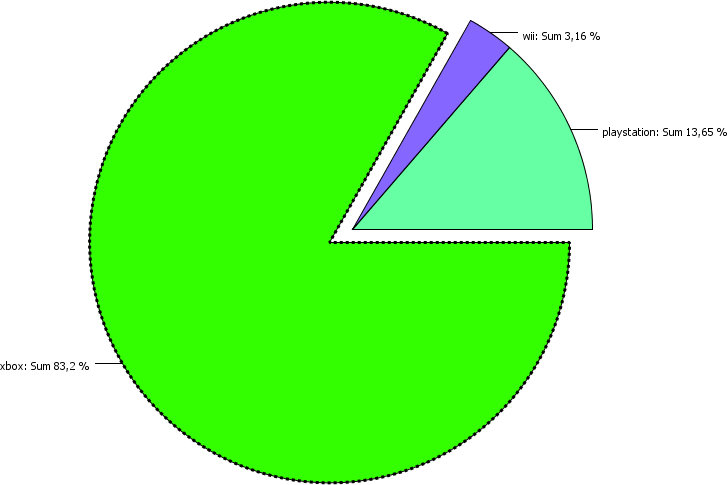
\includegraphics[width=\textwidth]{images/main_consoles}
    \caption{Part des vues selon la plateforme (console) du jeu}
    \label{fig:main_consoles}
\end{figure}

Nous remarquons à partir de la figure \ref{fig:main_categories} donc que la
catégorie \textbf{strategy} se détache des autres, prenant plus de 60 \% de la
part du nombre de vues des flux. Ceci correspond bien à nos attentes, vu que
Twitch est principalement connu pour des jeux développés pour PC, avec une
préférence pour les jeux de stratégie/roleplay (Starcraft, League of Legends,
etc...).

\begin{figure}[h]
    \centering
    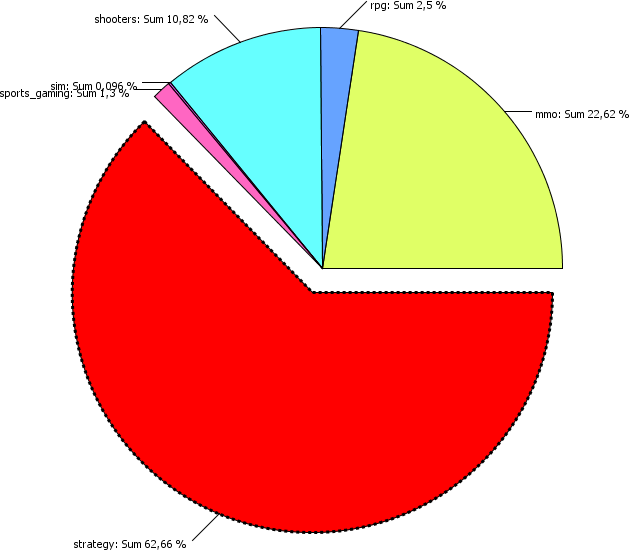
\includegraphics[width=\textwidth]{images/main_categories}
    \caption{Part des vues selon la catégorie du jeu}
    \label{fig:main_categories}
\end{figure}

\subsection{Les jeux vidéo populaires}
\begin{figure}[h]
    \centering
    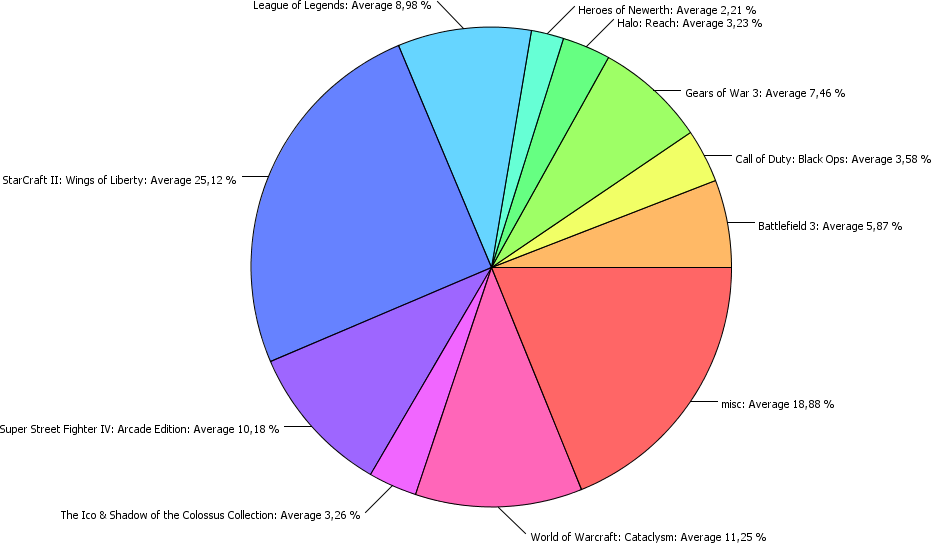
\includegraphics[width=\textwidth]{images/main_games}
    \caption{Part de vue en moyenne des jeux vidéo}
    \label{fig:main_games}
\end{figure}

Dans le jeu de données utilisé, la plupart des jeux étaient en doublons car ils
n'étaient pas tous orthographiés de la même façon (majuscules/minuscules,
espaces, ...). Nous n'avons pas pu, à cause de la taille des données, corriger
toutes les entrées afin d'unifier l'écriture des jeux. Les résultats ne sont
donc pas complètement exacts mais donnent tout de même une bonne approximation
de la réalité.

En tout il y a 160 jeux différents en comptant les doublons. Nous avons établi
la part de vue des différents jeux en groupant sur le champ \textit{meta-name}
et en sommant l'heuristique de popularité. Comme une grande quantité de jeu
était très minoritaire selon notre heuristique, nous avons regroupé ces
derniers (en seuillant la popularité) dans une seule catégorie \textit{misc}.

La figure \ref{fig:main_games} représente la popularité de chaque jeux.
L'ensemble des jeux \textit{misc} forment $19\%$ de popularité tandis que 10
autres jeux prennent les $80\%$ restant. Il y a donc une très grande disparité
dans les jeux vidéo et une petite minorité de 10 jeux écrasent totalement 150
autres jeux.

\begin{table}[c]
  \centering
   \caption{\label{tab:games_rank} Classement des 10 jeux les plus populaires
   sur la plateforme Twitch.}
   \begin{tabular}{|c|c|c|}
     \hline
     Position & Jeux vidéo & Part de popularité (en \%) \\
     \hline
     1 & StarCraft II & 25.12 \\
     2 & World of Warcraft : Cataclysm & 11.25 \\
     3 & Super Street Fighter IV & 10.18 \\
     4 & League of Legends & 8.98 \\
     5 & Gears of War & 7.46 \\
     6 & Battlefield 3 & 5.87 \\
     7 & Call of Duty : Black Ops & 3.58 \\
     8 & The Ico \& Shadow of Colossus Collection & 3.26 \\
     9 & Halo : Reach & 3.23 \\
     10 & Heroes of Newerth & 2.21 \\
     \hline
   \end{tabular}
\end{table}

Le tableau \ref{tab:games_rank} montre alors un classement des jeux les plus
populaires sur la plateforme Twitch.

\begin{figure}[h]
    \centering
    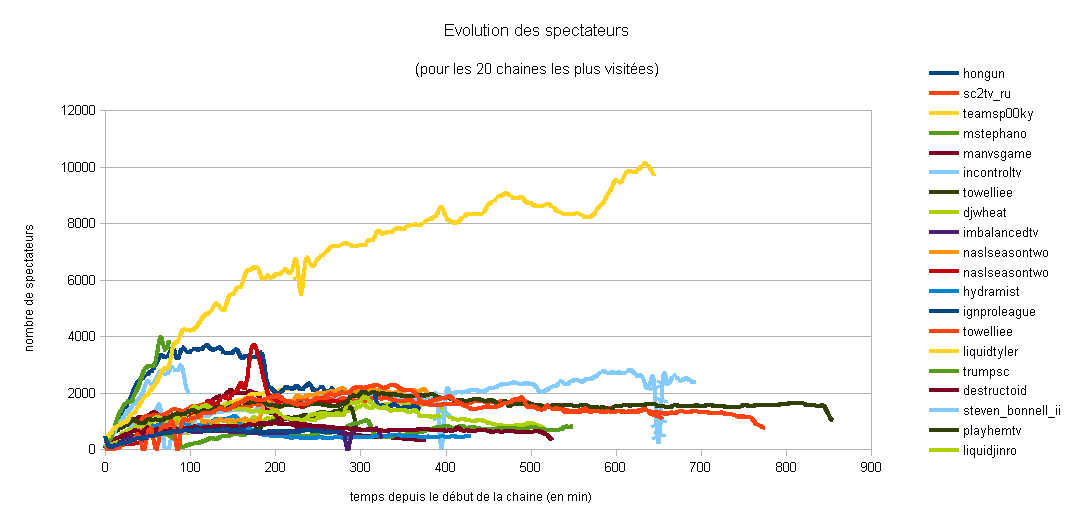
\includegraphics[width=\textwidth]{images/top_20_view_evolutions}
    \caption{}
\end{figure}

\section{Prédiction de l'audience d'un flux}

Un des intérêts majeur de cette étude est de pouvoir prédire l'audience d'un
flux à partir d'informations simples sur le flux, telles que la localisation,
la langue ou encore le type de jeu. \\

Nous nous sommes focalisés sur l'étude de la qualité d'un flux, ainsi que sa
localisation et sa langue, pour pouvoir prévoir la popularité du flux.

\subsection{Localisation/Langue}

Avant de démarrer, la première impression en observant le jeu de données, a été
le poids important des États-Unis dans l'audience de Twitch, vu que cette
plateforme a été développée là-bas. Ça n'a donc pas été surprenant de voir nos
différents calculs de clusters par localisation écrasés par le poids des
États-Unis. \\

En ce qui concerne la langue, le résultat est encore plus flagrant, la langue
anglaise est présente sur une majorité imposante des flux. Ce n'est donc pas
surprenant de ne pas pouvoir prévoir quoi que ce soit à partir de cette
information. \\

En conclusion, notre recherche de groupes ou de motifs récurrents à partir des
informations de localisation a été infructueuse. Peut-être qu'à partir
d'informations plus détaillées moins anonymes, avec par exemple la position
géographique approximative du joueur, nous sommes qu'il serait possible de
prédire l'audience du flux.

\subsection{Qualité}

\begin{figure}[h]
    \centering
    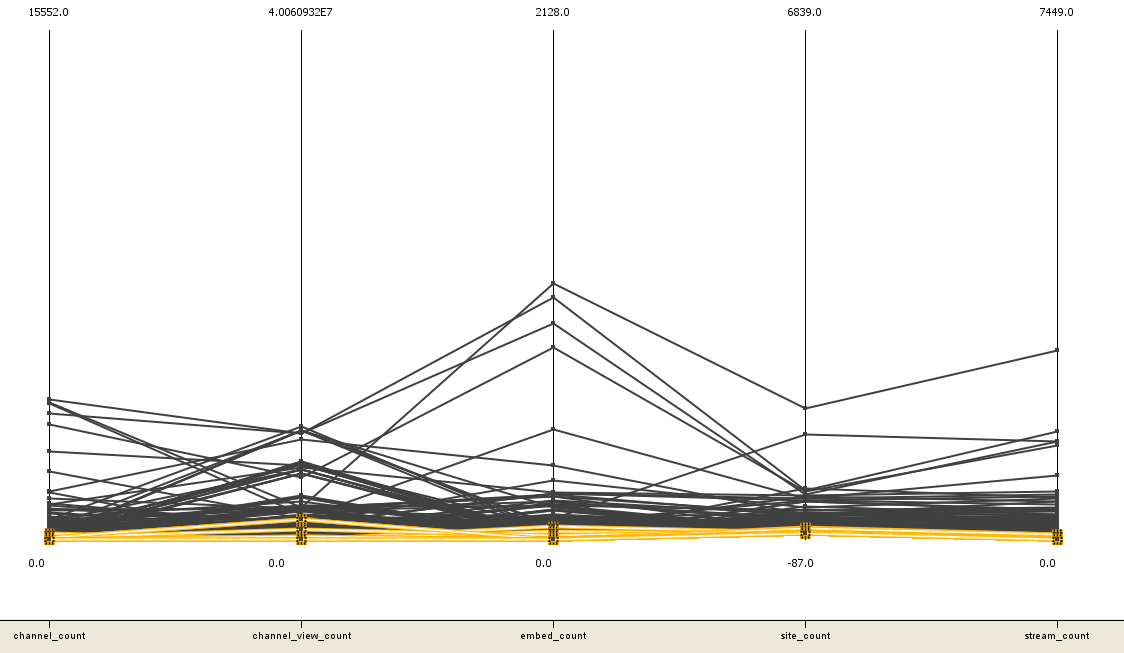
\includegraphics[width=\textwidth]{images/embed_enabled_influence}
    \caption{}
\end{figure}

\begin{figure}[h]
    \centering
    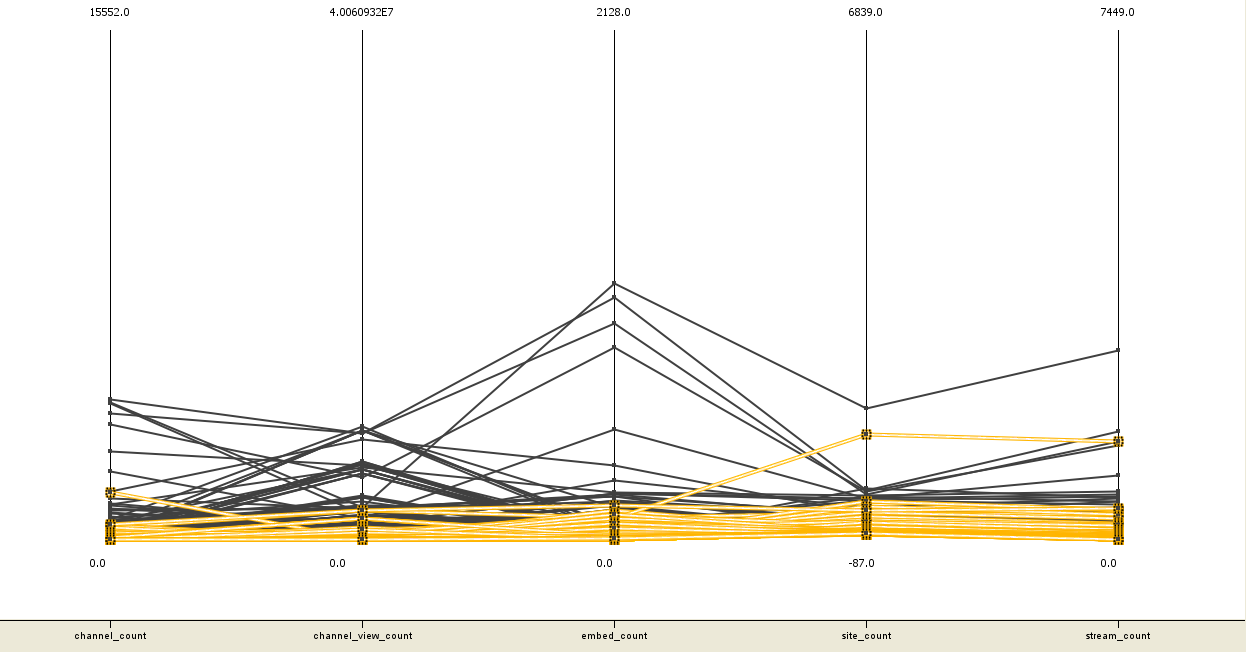
\includegraphics[width=\textwidth]{images/featured_influence}
    \caption{}
\end{figure}

% TODO

\section{Classement des "meilleurs" joueurs}

% TODO classement par tableau/graphe

\end{document}
